\documentclass[paper=a4, fontsize=11pt]{scrartcl}
\usepackage[T1]{fontenc}
\usepackage[utf8]{inputenc}
\usepackage{lmodern}
\usepackage{multirow}
\usepackage[table,xcdraw]{xcolor}
\usepackage[spanish]{babel}
\usepackage{cite}
\usepackage{amsmath,amsfonts,amsthm} % Math packages
\usepackage{graphics,graphicx, float} %para incluir imágenes y colocarlas
\usepackage[backref,colorlinks=true,linkcolor=black,urlcolor=blue,citecolor=blue]{hyperref} %Para crear enlaces en el pdf
\usepackage[noabbrev,spanish]{cleveref}
\usepackage{url}
\usepackage[shortlabels]{enumitem}
\usepackage{appendix}
\usepackage{eurosym}
\usepackage{epsfig}
\usepackage{caption}
\usepackage{subcaption}

\renewcommand{\appendixname}{Anexo}
\renewcommand{\appendixtocname}{Anexo}
\renewcommand{\appendixpagename}{Anexo}

\numberwithin{figure}{section} % Number figures within sections (i.e. 1.1, 1.2, 2.1, 2.2 instead of 1, 2, 3, 4)
\numberwithin{table}{section} % Number tables within sections (i.e. 1.1, 1.2, 2.1, 2.2 instead of 1, 2, 3, 4)
\newcommand{\horrule}[1]{\rule{\linewidth}{#1}} % Create horizontal rule command with 1 argument of height

\title{
    \normalfont \normalsize
    \textsc{{\bf Ingeniería de Servidores (2015-2016)} \\ Grado en Ingeniería Informática \\ Universidad de Granada} \\ [25pt] % Your university, school and/or department name(s)
    \horrule{0.5pt} \\[0.4cm] % Thin top horizontal rule
    \huge Memoria Práctica 5 \\ % The assignment title
    \horrule{2pt} \\[0.5cm] % Thick bottom horizontal rule
}
\author{Antonio de la Vega Jiménez }

%*************************************************************


\begin{document}

\maketitle % Muestra el Título
\newpage %inserta un salto de página
\tableofcontents % para generar el índice de contenidos
\listoffigures
\newpage
%*************************************************************

\section{Phoronix Suite}
\subsection{Cuestión 1}
\textit{Instale la aplicación. ¿Qué comando permite listar los benchmarks disponibles?}
\newline

 Para la instalación de Phoronix Suite he hecho uso de los comando mostrados en \cref{fig1}. Para listar los benchmarks disponibles se pueden usar la opción \texttt{list-available-tests}\cite{pho} de Phoronix Suite, como se indica en \cref{fig2}.
 
 \begin{figure}[H]
  \begin{center}
    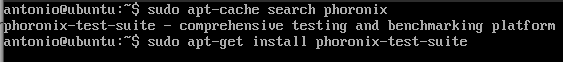
\includegraphics[width=1\textwidth]{imagenes/pho1}
    \caption{Comando para la instalación de Phoronix Suite en Ubuntu.}
    \label{fig1}
  \end{center}
\end{figure}

\begin{figure}[H]
  \begin{center}
    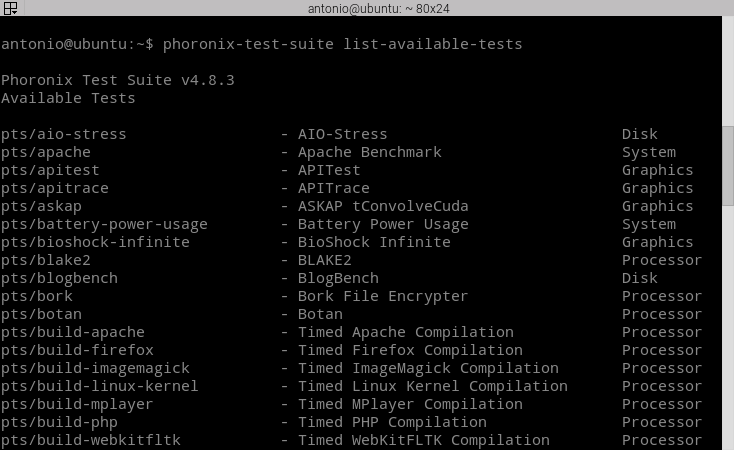
\includegraphics[width=1\textwidth]{imagenes/pho2}
    \caption{Uso del comando \texttt{list-available-tests} para ver los benchmarks disponibles.}
    \label{fig2}
  \end{center}
\end{figure}

\subsection{Cuestión opcional 1}
\textit{Seleccione, instale y ejecute uno, comente los resultados. Atención: no es lo mismo un benchmark que una suite, instale un benchmark.}
\newline

Para esta cuestión he instalado un benchmark llamado pts/n-queen, este benchmark es un programa que usa OpenMP y resuelve el problema de las N-Reinas ( Consiste en colocar un 18 reinas ( en este caso ) en un tablero sin que se amenacen ) en un tablero de tamaño 18 \cite{nr}. La instalación la he realizado como se indica en la \cref{fig13}, los resultados son los mostrados en las \crefrange{fig14}{fig15}.

\begin{figure}[H]
  \begin{center}
    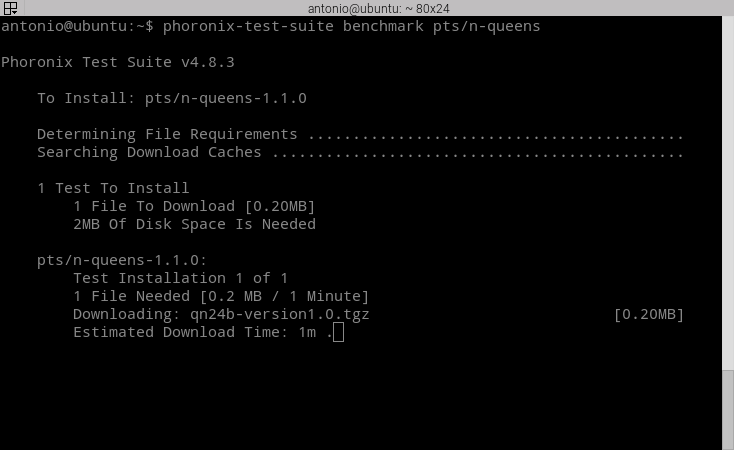
\includegraphics[width=1\textwidth]{imagenes/pho3}
    \caption{Comando para la instalación del benchmark.}
    \label{fig13}
  \end{center}
\end{figure}

\begin{figure}[H]
  \begin{center}
    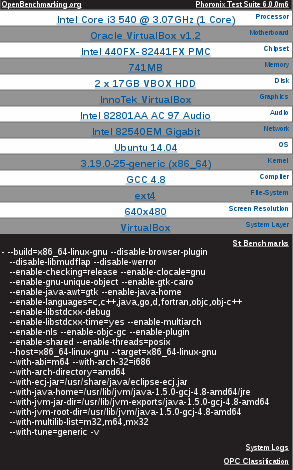
\includegraphics[width=0.4\textwidth]{imagenes/pho4}
    \caption{Información acerca del ordenador usado.}
    \label{fig14}
  \end{center}
\end{figure}

\begin{figure}[H]
  \begin{center}
    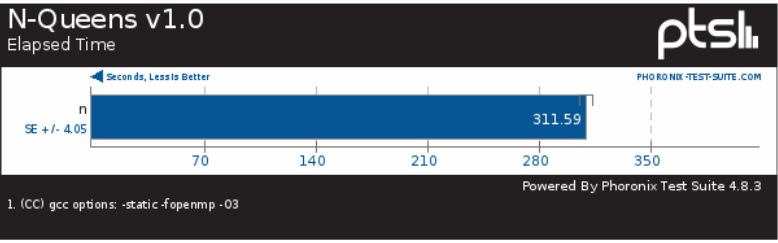
\includegraphics[width=1\textwidth]{imagenes/pho5}
    \caption{Resultado de la ejecución del benchmark, en el resultado se muestra el tiempo medio que se ha invertido en realizar el problema de las N-Reinas.}
    \label{fig15}
  \end{center}
\end{figure}

\section{Benchmarks y tests de estrés para webs}
\subsection{Apache benchmark}

\subsubsection{Cuestión 2}
\textit{De los parámetros que le podemos pasar al comando ¿Qué significa -c 5 ? ¿y -n 100? Monitorice la ejecución de ab contra alguna máquina (cualquiera) ¿cuántos procesos o hebras crea ab en el cliente?}
\newline

El comando \texttt{-c 5} significa que se ejecutaran 5 peticiones concurrentemente y el comando \texttt{-n 100} indica que se van a realizar 100 peticiones al servidor.\cite{ab} En el cliente solo se crea una hebra, como se puede ver con \texttt{top} ( \cref{fig11} ) o mirando en \texttt{/proc/pid\_ab/status} (\cref{fig12}).

\begin{figure}[H]
  \begin{center}
    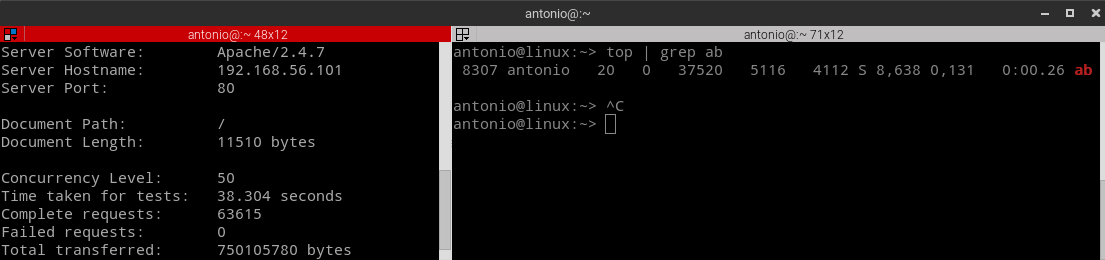
\includegraphics[width=1\textwidth]{imagenes/ab1}
    \caption{Comprobación del número de hebras mediante top.}
    \label{fig11}
  \end{center}
\end{figure}

\begin{figure}[H]
  \begin{center}
    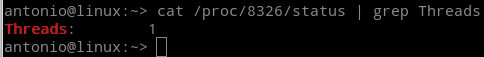
\includegraphics[width=1\textwidth]{imagenes/ab2}
    \caption{Comprobación del número de hebras mediante el archivo /proc/pid\_ab/status.}
    \label{fig12}
  \end{center}
\end{figure}


\subsubsection{Cuestión 3}
\textit{Ejecute ab contra a las tres máquinas virtuales (desde el SO anfitrión a las máquina virtuales de la red local) una a una (arrancadas por separado) y muestre y comente las estadísticas. ¿Cuál es la que proporciona mejores resultados? Fíjese en el número de bytes transferidos, ¿es igual para cada máquina?}
\newline

Para la ejecución del comando \texttt{ab -c 50 -n 100000 ip\_máquina:80/} la que proporciona mejores resultados es la de Windows Server (\cref{fig5})ya que IIS obtiene un rendimiento de 1828,63 peticiones por segundo y tiene un tiempo de respuesta de 0,547 ms, mientras que en Ubuntu ( Apache 2.4.7 ) (\cref{fig3}) se obtiene un rendimiento de 1730,06 peticiones por segundo y un tiempo de respuesta 0,578 ms, en última posición quedaría el servidor con CentOS (Apache 2.2.15 ) (\cref{fig4})  que consigue un rendimiento de 1338,26 peticiones por segundo y un tiempo de respuesta de 0,747 ms.\cite{ab} ( Ver figura \ref{fig6} )

\begin{figure}[H]
    \centering
    \begin{subfigure}[b]{0.45\textwidth}
        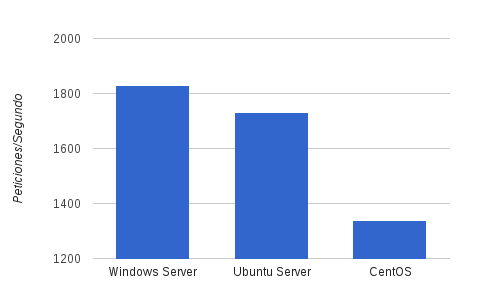
\includegraphics[width=\textwidth]{imagenes/g1}
        \caption{Peticiones por segundo.}
    \end{subfigure}
    \begin{subfigure}[b]{0.45\textwidth}
        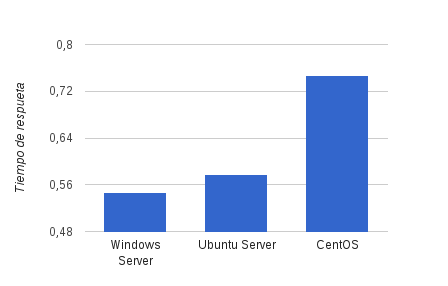
\includegraphics[width=\textwidth]{imagenes/g2}
        \caption{Tiempos de respuesta.}
    \end{subfigure}
    \caption{Comparativa servidores con ab}
    \label{fig6}
\end{figure}

\begin{figure}[H]
  \begin{center}
    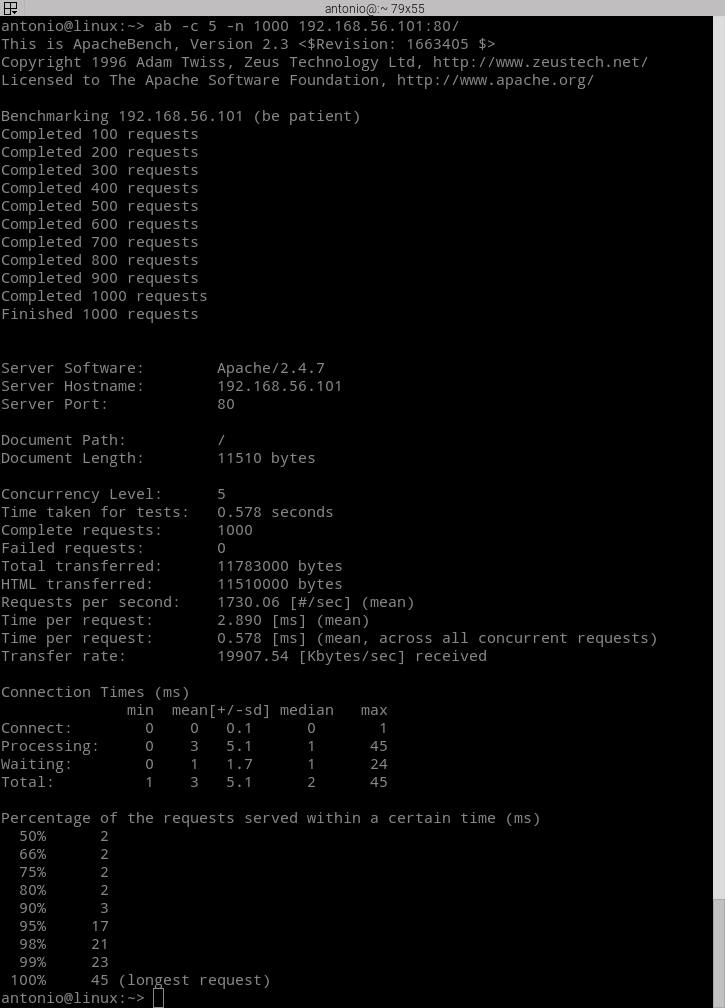
\includegraphics[width=1\textwidth]{imagenes/abub}
    \caption{Resultado de la ejecución de ab contra la maquina virtual de Ubuntu Server.}
    \label{fig3}
  \end{center}
\end{figure}
\begin{figure}[H]
  \begin{center}
    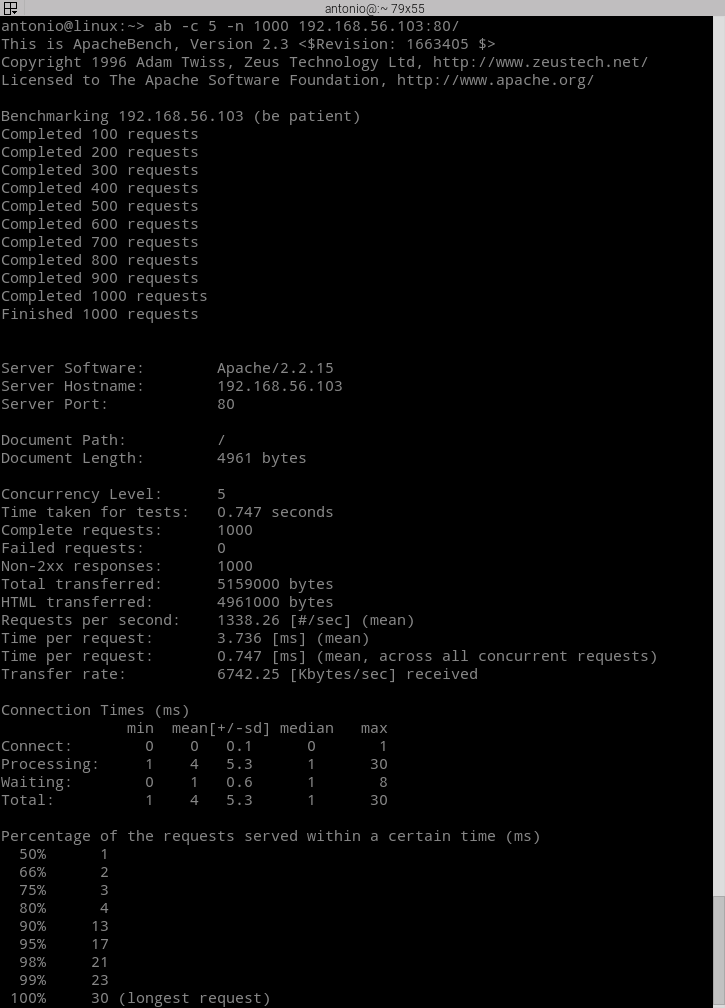
\includegraphics[width=1\textwidth]{imagenes/abce}
    \caption{Resultado de la ejecución de ab contra la maquina virtual de CentOS.}
    \label{fig4}
  \end{center}
\end{figure}
\begin{figure}[H]
  \begin{center}
    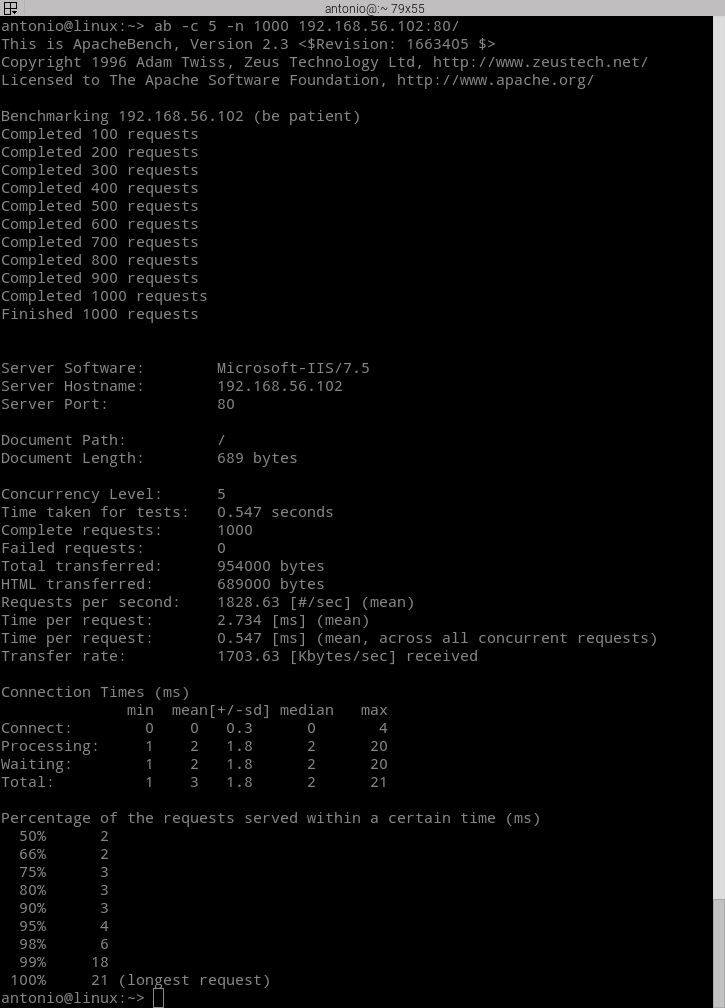
\includegraphics[width=1\textwidth]{imagenes/abwin}
    \caption{Resultado de la ejecución de ab contra la maquina virtual de Windows Server.}
    \label{fig5}
  \end{center}
\end{figure}

\subsection{Gatling}
\subsubsection{Cuestión opcional 2}
\textit{¿Qué es Scala? Instale Gatling y pruebe los escenarios por defecto.}

\subsection{Jmeter}
\subsubsection{Cuestión opcional 3}
\textit{Lea el artículo y elabore un breve resumen.}

\subsubsection{Cuestión 4}
\textit{Instale y siga el tutorial en \url{http://jmeter.apache.org/usermanual/build-web-test-plan.html} realizando capturas de pantalla y comentándolas. En vez de usar la web de jmeter, haga el experimento usando alguna de sus máquinas virtuales (Puede hacer una página sencilla, usar las páginas de phpmyadmin, instalar un CMS, etc.).}
\newline

Para realizar esta cuestión, en primer lugar, debemos conseguir JMeter, esto se puede hacer de dos formas, descargando el programa de \cite{jm} o mediante la orden \texttt{sudo apt-get install jmeter} en Ubuntu. Si optamos por el primer método deberemos extraer el archivo descargado y dentro, en la carpeta /bin, ejecutar \texttt{./jmeter.sh}. Una vez que tenemos JMeter funcionando podemos proceder a seguir el tutorial disponible en \cite{tut}, en mi caso voy a realizar peticiones a phpMyAdmin. El proceso de configuración se puede ver en las \crefrange{fig7}{fig10}.

\begin{figure}[H]
  \begin{center}
    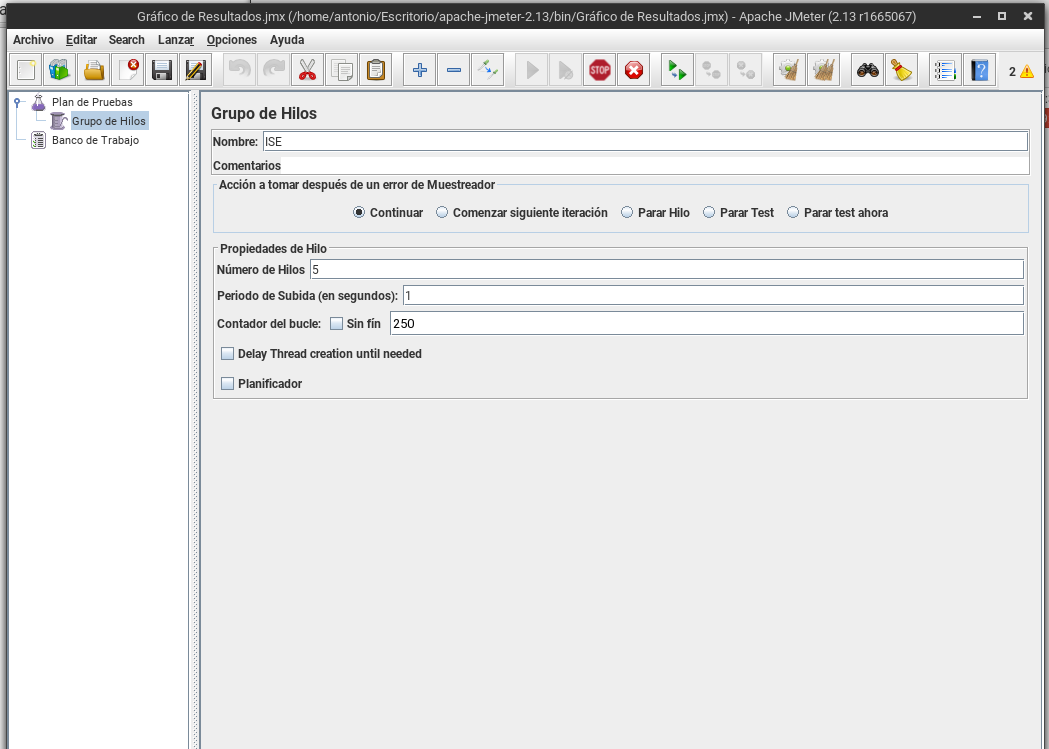
\includegraphics[width=0.7\textwidth]{imagenes/jm1}
    \caption{Añadimos un grupo de threads ( Thread Group o Grupo de Hilos ) que simularan los usuarios, en esta caso se configuran 5 usuarios y se repetirá el 250 veces.}
    \label{fig7}
  \end{center}
\end{figure}

\begin{figure}[H]
  \begin{center}
    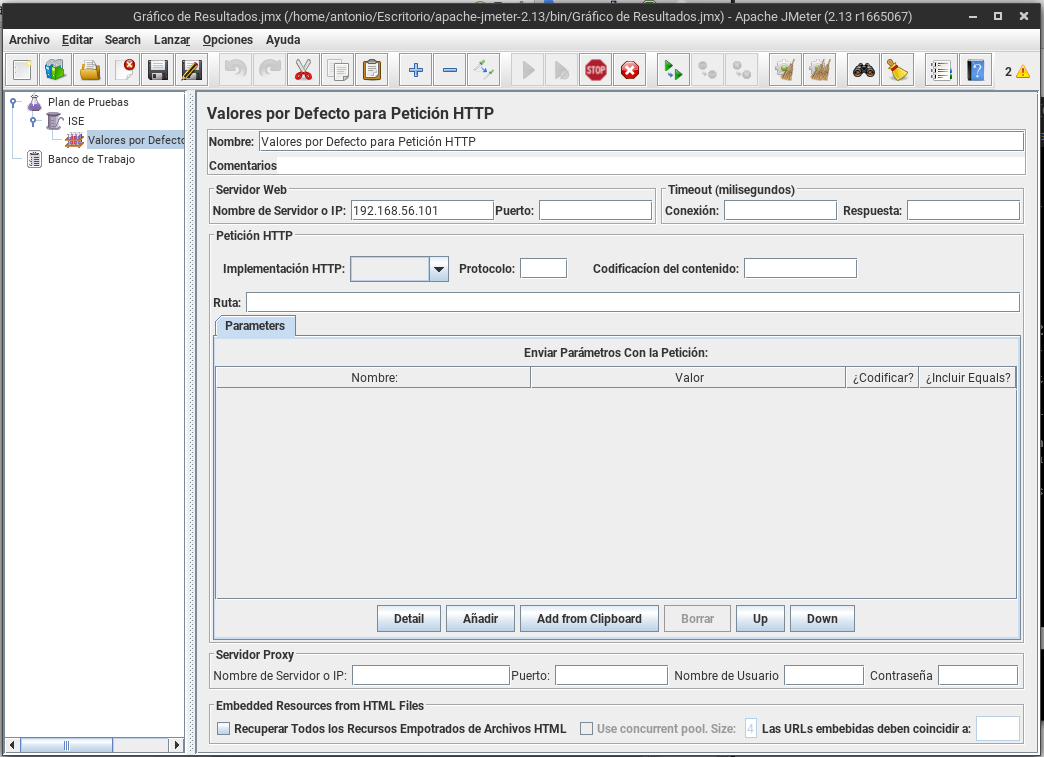
\includegraphics[width=0.7\textwidth]{imagenes/jm2}
    \caption{Añadimos los valores por defecto para las peticiones HTTP, en este caso de indica la IP de mi servidor.}
    \label{fig8}
  \end{center}
\end{figure}

\begin{figure}[H]
  \begin{center}
    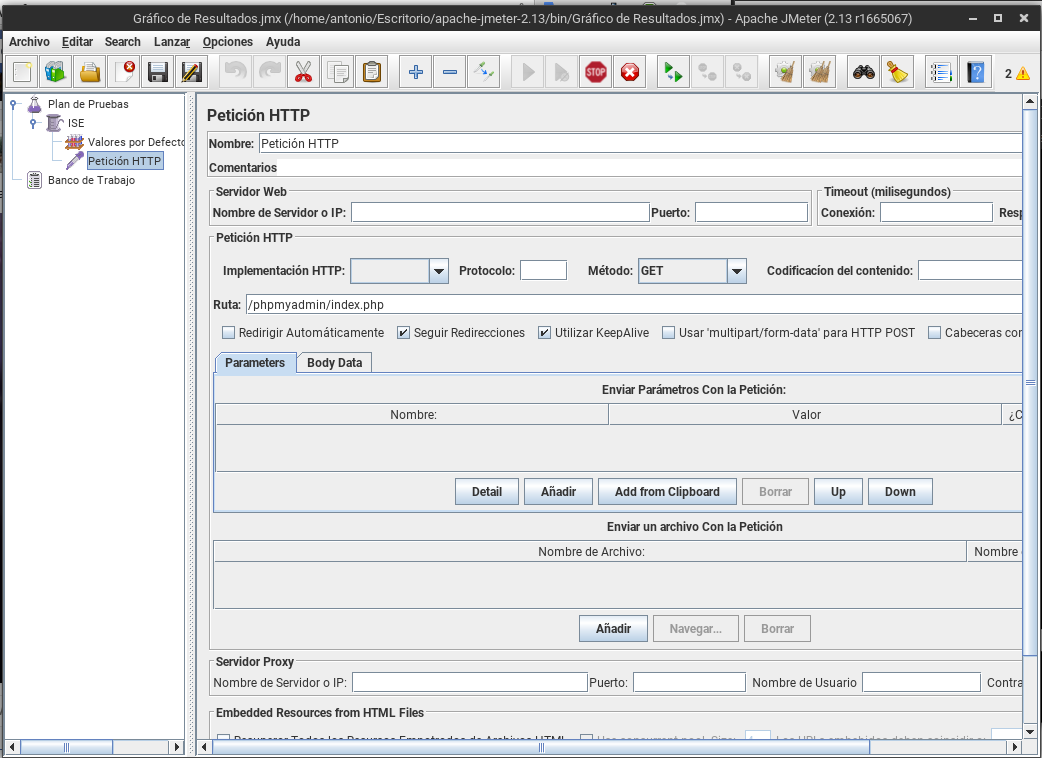
\includegraphics[width=0.7\textwidth]{imagenes/jm3}
    \caption{Se añade la petición HTTP que se va a realizar, en este caso un petición a la pagina de login de phpMyAdmin.}
    \label{fig9}
  \end{center}
\end{figure}

\begin{figure}[H]
  \begin{center}
    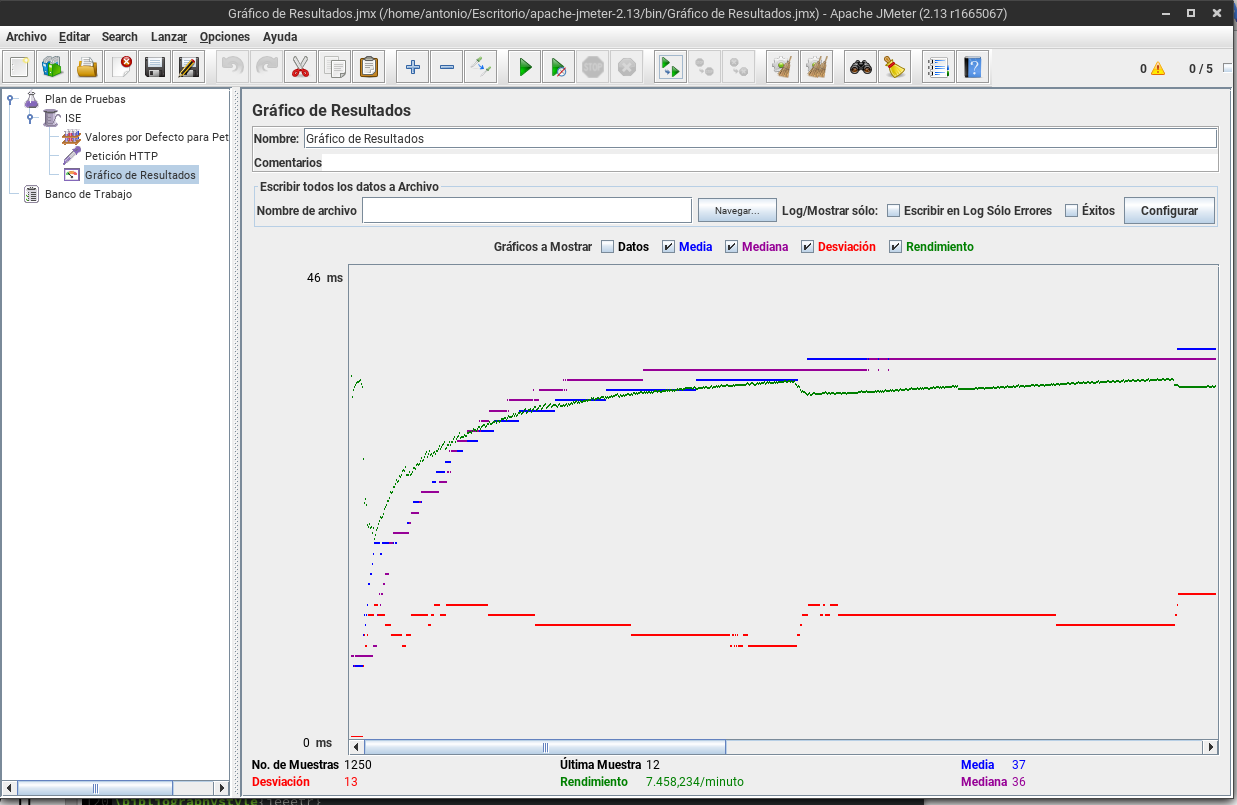
\includegraphics[width=0.7\textwidth]{imagenes/jm4}
    \caption{Añadimos un gráfico de resultados para poder ver el resultado de la ejecución del test. En este caso se puede ver que al principio el rendimiento del servidor va subiendo y luego se estabiliza.}
    \label{fig10}
  \end{center}
\end{figure}



\section{Benchmarks para Windows}
\subsection{AIDA64 (Antiguo Everest)}

\subsubsection{Cuestión opcional 4}
\textit{Seleccione un benchmark entre SisoftSandra y Aida.
Ejecútelo y muestre capturas de pantalla comentando los resultados.}

\section{Más benchmarks}
\subsection{Cuestión 5}
\textit{Cuestión 5: Programe un benchmark usando el lenguaje que desee. El benchmark debe incluir:
\begin{enumerate}
  \item Objetivo del benchmark
  \item Métricas (unidades, variables, puntuaciones, etc.)
  \item Instrucciones para su uso
  \item Ejemplo de uso analizando los resultados
\end{enumerate}}
%*************************************************************
\newpage
\bibliographystyle{ieeetr}
\bibliography{citas}

\end{document}
